% Options for packages loaded elsewhere
\PassOptionsToPackage{unicode}{hyperref}
\PassOptionsToPackage{hyphens}{url}
\PassOptionsToPackage{dvipsnames,svgnames*,x11names*}{xcolor}
%
\documentclass[
  a4paper,
]{article}
\usepackage{amsmath,amssymb}
\usepackage{lmodern}
\usepackage{setspace}
\usepackage{ifxetex,ifluatex}
\ifnum 0\ifxetex 1\fi\ifluatex 1\fi=0 % if pdftex
  \usepackage[T1]{fontenc}
  \usepackage[utf8]{inputenc}
  \usepackage{textcomp} % provide euro and other symbols
\else % if luatex or xetex
  \usepackage{unicode-math}
  \defaultfontfeatures{Scale=MatchLowercase}
  \defaultfontfeatures[\rmfamily]{Ligatures=TeX,Scale=1}
  \setmainfont[]{Lato}
\fi
% Use upquote if available, for straight quotes in verbatim environments
\IfFileExists{upquote.sty}{\usepackage{upquote}}{}
\IfFileExists{microtype.sty}{% use microtype if available
  \usepackage[]{microtype}
  \UseMicrotypeSet[protrusion]{basicmath} % disable protrusion for tt fonts
}{}
\usepackage{xcolor}
\IfFileExists{xurl.sty}{\usepackage{xurl}}{} % add URL line breaks if available
\IfFileExists{bookmark.sty}{\usepackage{bookmark}}{\usepackage{hyperref}}
\hypersetup{
  pdftitle={Pressure for rapid and accurate mate recognition promotes avian-perceived plumage sexual dichromatism in true thrushes (genus: Turdus)},
  pdfauthor={Alec B. Luro1*, Mark E. Hauber1},
  colorlinks=true,
  linkcolor=blue,
  filecolor=Maroon,
  citecolor=blue,
  urlcolor=Blue,
  pdfcreator={LaTeX via pandoc}}
\urlstyle{same} % disable monospaced font for URLs
\usepackage[margin=1in]{geometry}
\usepackage{graphicx}
\makeatletter
\def\maxwidth{\ifdim\Gin@nat@width>\linewidth\linewidth\else\Gin@nat@width\fi}
\def\maxheight{\ifdim\Gin@nat@height>\textheight\textheight\else\Gin@nat@height\fi}
\makeatother
% Scale images if necessary, so that they will not overflow the page
% margins by default, and it is still possible to overwrite the defaults
% using explicit options in \includegraphics[width, height, ...]{}
\setkeys{Gin}{width=\maxwidth,height=\maxheight,keepaspectratio}
% Set default figure placement to htbp
\makeatletter
\def\fps@figure{htbp}
\makeatother
\setlength{\emergencystretch}{3em} % prevent overfull lines
\providecommand{\tightlist}{%
  \setlength{\itemsep}{0pt}\setlength{\parskip}{0pt}}
\setcounter{secnumdepth}{-\maxdimen} % remove section numbering
\usepackage[left]{lineno}
\linenumbers
\usepackage{graphicx}
\usepackage{booktabs}
\usepackage{caption}
\usepackage{lscape}
\ifluatex
  \usepackage{selnolig}  % disable illegal ligatures
\fi
\newlength{\cslhangindent}
\setlength{\cslhangindent}{1.5em}
\newlength{\csllabelwidth}
\setlength{\csllabelwidth}{3em}
\newenvironment{CSLReferences}[2] % #1 hanging-ident, #2 entry spacing
 {% don't indent paragraphs
  \setlength{\parindent}{0pt}
  % turn on hanging indent if param 1 is 1
  \ifodd #1 \everypar{\setlength{\hangindent}{\cslhangindent}}\ignorespaces\fi
  % set entry spacing
  \ifnum #2 > 0
  \setlength{\parskip}{#2\baselineskip}
  \fi
 }%
 {}
\usepackage{calc}
\newcommand{\CSLBlock}[1]{#1\hfill\break}
\newcommand{\CSLLeftMargin}[1]{\parbox[t]{\csllabelwidth}{#1}}
\newcommand{\CSLRightInline}[1]{\parbox[t]{\linewidth - \csllabelwidth}{#1}\break}
\newcommand{\CSLIndent}[1]{\hspace{\cslhangindent}#1}

\title{Pressure for rapid and accurate mate recognition promotes
avian-perceived plumage sexual dichromatism in true thrushes (genus:
\emph{Turdus})}
\author{Alec B. Luro\textsuperscript{1}*, Mark E.
Hauber\textsuperscript{1}}
\date{\textsuperscript{1} Department of Evolution, Ecology and Behavior,
School of Integrative Biology, University of Illinois at
Urbana-Champaign *alec.b.luro@gmail.com}

\begin{document}
\maketitle

\setstretch{1.5}
\hypertarget{abstract}{%
\section{Abstract}\label{abstract}}

Ecological conditions limiting the time to find a compatible mate or
increasing the difficulty in doing so likely promote the evolution of
traits used for species and mate recognition. Conspicuous traits that
signal an individual's species, sex, and breeding status reduce the
challenge of identifying a compatible conspecific mate, and should be
more common in migratory rather than sedentary species, species with
shorter breeding seasons, and species breeding under high sympatry with
many closely-related heterospecifics. Here, we tested this recognition
hypothesis for promoting plumage sexual dichromatism in the true
thrushes (\emph{Turdus} spp.), a large and diverse genus of passerine
birds. We used receptor-noise limited models of avian vision to quantify
avian-perceived chromatic and achromatic visual contrasts between male
and female plumage patches and tested the influence of breeding season
length, spatial distribution, and sympatry with other \emph{Turdus}
species on plumage dichromatism. As predicted, we found that 1) true
thrush species with migratory behaviour have greater plumage sexual
dichromatism than non-migratory species, 2) species with longer breeding
seasons have less plumage sexual dichromatism, and 3) greater numbers of
\emph{Turdus} thrush species breeding in sympatry is associated with
more plumage sexual dichromatism. These results suggest that social
recognition systems, including species and mate recognition, play a
prominent role in the evolution of plumage sexual dichromatism in true
thrushes.

\hypertarget{keywords}{%
\subsection{Keywords}\label{keywords}}

\emph{achromatic}, \emph{chromatic}, \emph{dichromatism},
\emph{plumage}, \emph{mate recognition}

\hypertarget{introduction}{%
\section{Introduction}\label{introduction}}

Species recognition is necessary in sexually reproducing lineages for
individuals to find compatible mates and produce viable offspring
{[}\protect\hyperlink{ref-andersson1994}{1},\protect\hyperlink{ref-groning2008}{2}{]}.
Conspicuous traits signaling species and sex identity increase the ease
and speed of mate recognition by reducing the effort, error, and time
involved when searching for compatible mates and lessen the likelihood
of mating with heterospecifics
{[}\protect\hyperlink{ref-pfennig2012}{3}{]}. Traits used in species and
mate recognition may also serve as signals of status to conspecifics and
reduce costly conflicts over resources and mates
{[}\protect\hyperlink{ref-west-eberhard1983}{4}{]}. Accordingly,
distinct traits facilitating mate recognition should be more likely to
arise and be maintained under conditions that increase both the
difficulty of finding a compatible mate and degree of resource
competition among conspecifics and closely-related species. Conditions
likely to favour traits signaling individuals' species, sex, and
breeding status include higher sympatry with many closely-related
species, limited time to find compatible breeding mates, and lower rates
of encounter with potential breeding mates
{[}\protect\hyperlink{ref-andersson1994}{1}{]}.

In birds, plumage colour is a highly conspicuous trait signaling species
and (often) sex identity
{[}\protect\hyperlink{ref-martin2015a}{5},\protect\hyperlink{ref-bitton2016}{6}{]}.
Plumage sexual dichromatism, or the distinct set of differences in the
appearance of male and female feather colours and patterns, is common in
birds and is usually attributed to different natural and sexual
selection pressures on males and females
{[}\protect\hyperlink{ref-martin1996}{7}--\protect\hyperlink{ref-dunn2015}{11}{]}.
Plumage sexual dichromatism results in a visibly perceivable trait
useful for recognizing an individual's species, sex, and breeding status
(e.g., in species with sex-specific delayed plumage maturation, see
{[}\protect\hyperlink{ref-hawkins2012}{12}{]}), reducing the time and
effort expended to identify a suitable mate
{[}\protect\hyperlink{ref-hamilton1961}{13},\protect\hyperlink{ref-saetre1992}{14}{]}.
Evidence in favour of this recognition hypothesis for sexual
dichromatism in birds includes a positive association of greater plumage
sexual dichromatism with migratory behaviour and shorter breeding
seasons {[}\protect\hyperlink{ref-badyaev2003}{9}{]}, both of which
reduce the amount of time available to search and find suitable mates
and successfully breed. Additional support for the recognition
hypothesis includes a consistent pattern of greater plumage sexual
dichromatism and plumage colour elaboration in avian species that reside
on mainland continents and have large geographic ranges in comparison to
species that do not migrate, reside on islands, and have limited
breeding ranges
{[}\protect\hyperlink{ref-dale2015}{10},\protect\hyperlink{ref-friedman2009}{15}--\protect\hyperlink{ref-kearns2020}{23}{]}.

Moreover, plumage sexual dichromatism likely plays a role in
hybridization avoidance via reproductive character displacement to
facilitate species and mate recognition, especially among
closely-related species. For example, in \emph{Ficedula} flycatchers,
female choice selects for divergent male plumage colouration across
populations and species, leading to male character displacement and
reduced rates of interspecific hybridization
{[}\protect\hyperlink{ref-alatalo1994}{24}--\protect\hyperlink{ref-laaksonen2015}{26}{]}.
More broadly and across taxa, greater plumage dichromatism is positively
associated with higher breeding sympatry with closely-related
heterospecifics. Among a large sample of passerine sister species pairs,
transitions from allopatry to parapatry and increases in geographic
range overlaps are positively correlated with greater plumage
dichromatism {[}\protect\hyperlink{ref-cooney2017}{27}{]}. Greater
plumage sexual dichromatism has also been found to be positively
associated with greater avian species divergence and richness
{[}\protect\hyperlink{ref-seddon2013}{28},\protect\hyperlink{ref-cooney2019}{29}{]}.
Among passerine sister species pairs, more pronounced changes in male
rather than female plumage colouration in sexually-dichromatic species
suggest that female choice and male-male competition often lead to
concurrent increases in sexual dichromatism and speciation events
{[}\protect\hyperlink{ref-seddon2013}{28}{]}. Therefore, plumage sexual
dichromatism may be a selected trait for facilitating species and mate
recognition when closely-related species have sympatric breeding ranges
{[}\protect\hyperlink{ref-martin2015a}{5},\protect\hyperlink{ref-martin2010}{30}{]}.

True thrushes (\emph{Turdus} spp.) are an exceptionally diverse
monophyletic genus of passerine birds consisting of about
\textasciitilde86 species distributed across the globe
(\protect\hyperlink{fig:fig-01-turdus-ranges}{Fig. 1}). The true
thrushes are an ideal passerine clade for examining the recognition
hypothesis for plumage sexual dichromatism because plumage sexual
dichromatism and migratory behaviours vary substantially between species
and sexual dichromatism has evolved multiple times in thrushes across
the world
{[}\protect\hyperlink{ref-clement2000}{31},\protect\hyperlink{ref-nagy2019}{32}{]}.
Hybridization also occurs in some, but not all, \emph{Turdus} species,
indicating that some sympatric \emph{Turdus} species can successfully
interbreed. A particulary well-documented example of hybridization in
true thrushes occurs at large hybrid zone between four \emph{Turdus}
species (\emph{T. atrogularis}, \emph{T. eunomus}, \emph{T. naumanni},
\emph{T. ruficollis}) in north-central Asia
{[}\protect\hyperlink{ref-mccarthy2006}{33}{]}. Further, plumage sexual
dichromatism in true thrushes often coincides with age and breeding
status in male thrushes. Delayed plumage maturation in males is common
among true thrushes
{[}\protect\hyperlink{ref-escalona-segura1997}{34}--\protect\hyperlink{ref-ligon2013}{36}{]},
where males have ``female-like'' plumage colouration during their first
breeding season and develop typical breeding adult male plumage for
subsequent breeding seasons. The presence of delayed plumage maturation
and distinct juvenal plumage may serve as a signal of a young male's
sexual immaturity in order to reduce levels conspecific aggression from
older adults {[}\protect\hyperlink{ref-ligon2013}{36}{]} and also
suggests that female thrushes prefer older males with prominent adult
plumage as breeding mates.

Overall, ecological conditions that increase the time and degree of
difficulty in finding a suitable conspecific mate should select for
phenotypic traits that reliably signal species and sex identity. Across
various bird lineages, greater plumage dichromatism is present in
species that are i) migratory rather than nonmigratory, ii) have shorter
breeding seasons, iii) live on mainlands rather than islands, iv) have
larger breeding ranges (distributions), and v) breed in sympatry with
more closely-related species. These patterns suggest that ecological
circumstances where rapid and accurate mate recognition is challenging
strongly favour the evolution and maintenance of prominent plumage
sexual dichromatism in birds. Here, we test these predictions of the
recognition hypothesis for plumage sexual dichromatism by evaluating the
potential influences of breeding timing, spacing, and sympatry on
plumage dichromatism in \emph{Turdus} thrushes
(\protect\hyperlink{fig:fig:02-hypotheses}{Fig. 2}).

\begin{figure}
\hypertarget{fig:fig-01-turdus-ranges}{%
\centering
\includegraphics{Figures/01_turdus_species_worldmap_with_HBW.png}
\caption{Breeding ranges of all recognized \emph{Turdus} species from
BirdLife International, with representative species' males and females
shown for species with plumage sexual dichromatism. The color scale
indicates the number of \emph{Turdus} thrush species in sympatry with
overlapping breeding ranges. Illustrations used with permission from HBW
Alive/Lynx Edicions}\label{fig:fig-01-turdus-ranges}
}
\end{figure}

\begin{figure}
\hypertarget{fig:fig:02-hypotheses}{%
\centering
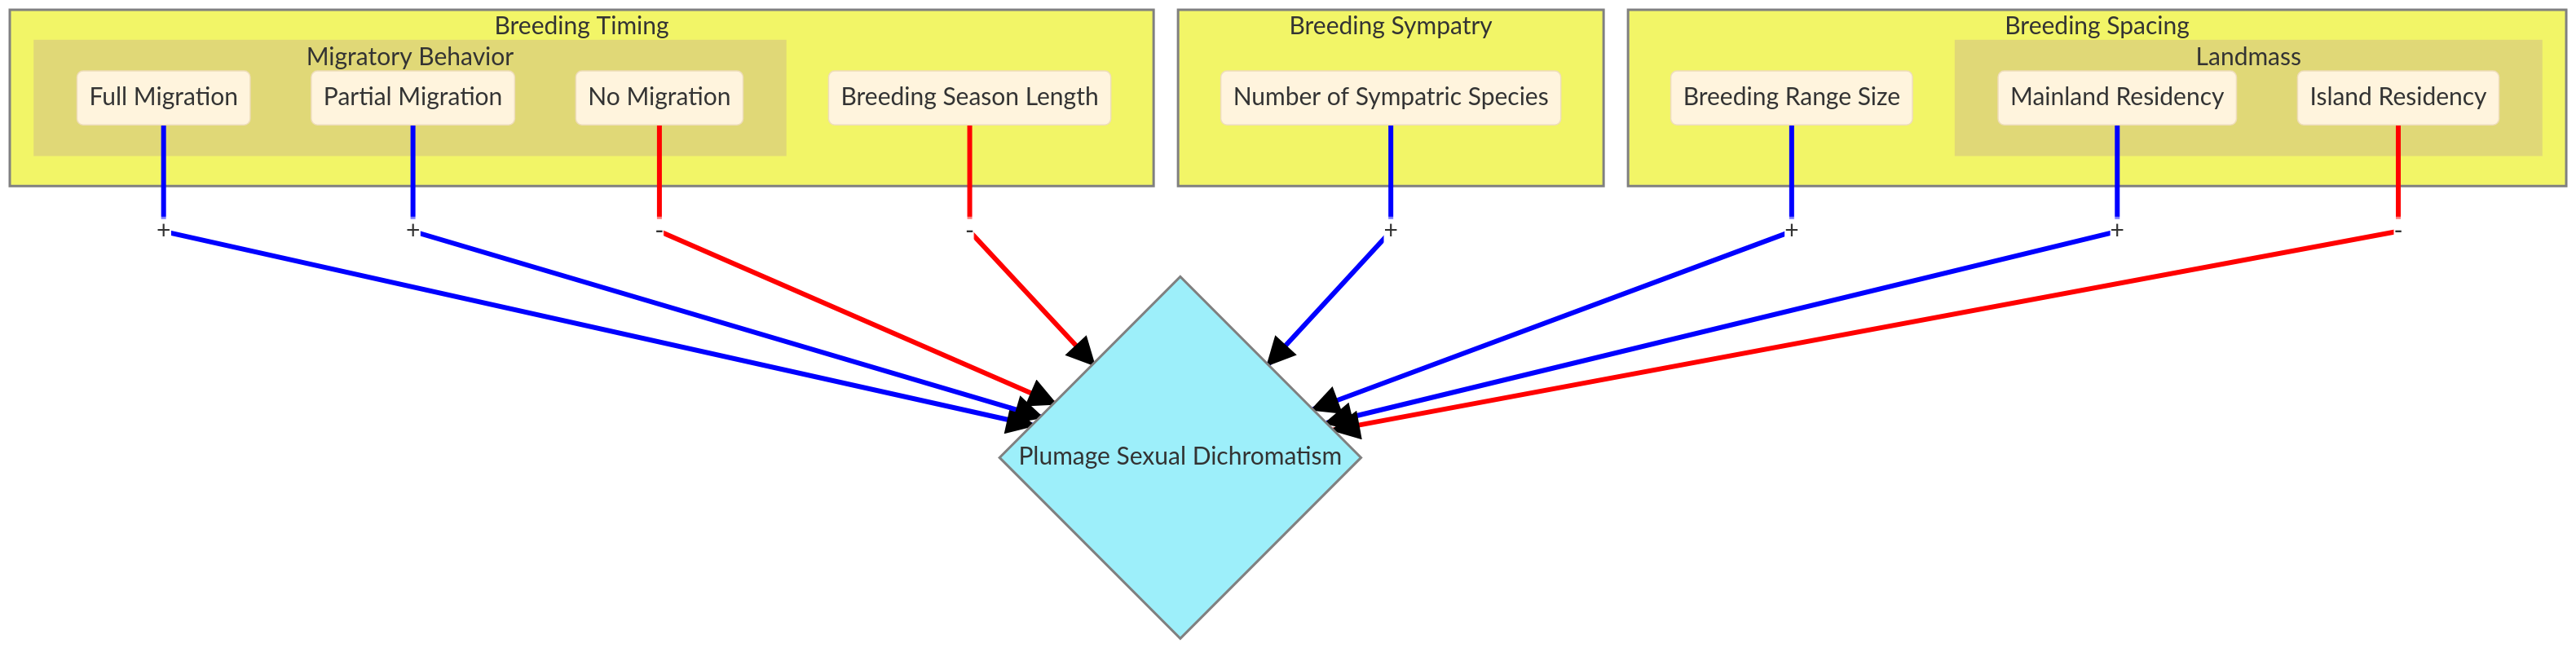
\includegraphics{Figures/hypothesis-figure-mermaid.png}
\caption{Hypotheses and predictions for each model (large yellow boxes).
Arrow colours indicate predicted correlation, positive (blue) and
negative (red)}\label{fig:fig:02-hypotheses}
}
\end{figure}

\hypertarget{methods}{%
\section{Methods}\label{methods}}

Initial pre-registration of the study's methods and analyses are
available on \href{https://osf.io/zum6d}{Open Science Framework}
{[}\protect\hyperlink{ref-luro2019}{37}{]}.

\hypertarget{plumage-sexual-dichromatism}{%
\subsection{\texorpdfstring{\emph{Plumage sexual
dichromatism}}{Plumage sexual dichromatism}}\label{plumage-sexual-dichromatism}}

A total of N=77 \emph{Turdus} thrush species (approximately
\textasciitilde89\% of all known true thrush species) were sampled for
plumage spectral reflectance using prepared bird skin specimens at the
American Museum of Natural History in New York City and the Field Museum
in Chicago, USA. Reflectance measurements spanning 300-700nm were taken
in triplicate from the belly, breast, throat, crown, and mantle plumage
patches {[}\protect\hyperlink{ref-andersson2006}{38}{]} of each
individual. N=3 male and N=3 female individuals were measured for most
species (exceptions: \emph{T. lawrencii}, N=2 males and N=2 females;
\emph{T. swalesi}, N=1 male and N=1 female). Reflectance spectra were
measured using a 400 μm fiber optic reflection probe fitted with a
rubber stopper to maintain a consistent measuring distance of 3 mm and
area of 2 mm2 at a 90° angle to the surface of the feather patch.
Measurements were taken using a JAZ spectrometer with a pulsed-xenon
light source (Ocean Optics, Dunedin, USA) and we used a diffuse 99\%
reflectance white standard (Spectralon WS-1-SL, Labsphere, North Sutton
NH, USA).

We applied a receptor-noise limited visual model
{[}\protect\hyperlink{ref-vorobyev1998}{39}{]} of the European Blackbird
(\emph{T. merula}) visual system
{[}\protect\hyperlink{ref-hart2000}{40}{]} in the \emph{pavo}
{[}\protect\hyperlink{ref-maia2019}{41}{]}⁠ package in R v4.0.0
{[}\protect\hyperlink{ref-rcoreteam2020}{42}{]}⁠ to calculate
avian-perceived chromatic and achromatic visual contrast (in units of
``Just-Noticeable Differences'',or JNDs) of male vs.~female plumage
patches for all sampled \emph{Turdus} species. Chromatic and achromatic
JNDs were calculated for male-female pairs within each species (i.e.,
N=9 JND values calculated per patch for each species where N=3 males and
N=3 females sampled), and then JND values were averaged for each
species' respective plumage patches. Under ideal laboratory conditions,
1 JND is generally considered to be the discriminable threshold past
which an observer is predicted to be able to perceive the two colours as
different. However, natural light environments vary both spatially and
temporally {[}\protect\hyperlink{ref-endler1993}{43}{]}⁠, bringing into
question the accuracy of a 1 JND threshold for generalizing visual
contrast under natural conditions. Therefore, we calculated the total
number of sexually-dichromatic plumage patches per species (out of N=5
measured patches) as the number of plumage patches with average JND
values \textgreater{} 1, 2, or 3 to account for uncertainty in visual
discrimination thresholds due to variation in psychophysical and ambient
lighting conditions affecting the strength of between-sex plumage visual
contrast {[}\protect\hyperlink{ref-kemp2015}{44}{]}⁠. Additionally, we
modeled the number of divergent plumage patches (at the three different
JND thresholds listed above) within sexes and between different
sympatric species under different levels of breeding range overlap (10\%
increments between 0-90\%; Fig. S1).

\hypertarget{life-history-data}{%
\subsection{\texorpdfstring{\emph{Life History
Data}}{Life History Data}}\label{life-history-data}}

\hypertarget{breeding-timing-model}{%
\subsubsection{\texorpdfstring{\emph{Breeding Timing
Model}}{Breeding Timing Model}}\label{breeding-timing-model}}

We collected data on migration behaviour and breeding season length from
\emph{Thrushes} {[}\protect\hyperlink{ref-clement2000}{31}{]} and the
\emph{Handbook of the Birds of the World}
{[}\protect\hyperlink{ref-delhoyo2017}{45}{]}⁠. We assigned three
different kinds of migratory behaviour: 1) \emph{full migration} when a
species description clearly stated that a species ``migrates'', 2)
\emph{partial migration} when a species was described to have
``altitudinal migration'', ``latitudinal migration'' or ``movement
during non-breeding season'', or 3) \emph{sedentary} when a species was
described as ``resident'' or ``sedentary''. Breeding season length was
defined as the number of months the species breeds each year.

\hypertarget{breeding-sympatry-model}{%
\subsubsection{\texorpdfstring{\emph{Breeding Sympatry
Model}}{Breeding Sympatry Model}}\label{breeding-sympatry-model}}

Species' breeding ranges were acquired from \emph{BirdLife
International}
{[}\protect\hyperlink{ref-birdlifeinternationalandhandbookofthebirdsoftheworld2018}{46}{]}⁠.
We calculated congener breeding range overlaps (as percentages) using
the \emph{letsR} package in R
{[}\protect\hyperlink{ref-vilela2015}{47}{]}⁠. We then calculated the
number of sympatric species as the number of congeners with breeding
ranges that overlap \textgreater30\% with the focal species' breeding
range {[}\protect\hyperlink{ref-cooney2017}{27}{]}. Comparisons of the
number of sexually-dimorphic plumage patches vs.~the number of sympatric
species among different breeding range overlap thresholds are provided
in Supplementary Figure 2.

\hypertarget{breeding-spacing-model}{%
\subsubsection{\texorpdfstring{\emph{Breeding Spacing
Model}}{Breeding Spacing Model}}\label{breeding-spacing-model}}

Species' breeding range sizes (in km2) were acquired using the
\emph{BirdLife International} breeding range maps. Species' island
vs.~mainland residence was also determined using breeding ranges from
\emph{BirdLife International}. Mainland residence was assigned if the
species had a breeding range on any continent and Japan. Island
residence was assigned to species having a breeding range limited to a
non-continental landmass entirely surrounded by a marine body of water.

\hypertarget{statistical-modeling}{%
\subsection{\texorpdfstring{\emph{Statistical
modeling}}{Statistical modeling}}\label{statistical-modeling}}

We used phylogenetically-corrected Bayesian multilevel logistic
regression models using the \emph{brms} v2.13.0 package
{[}\protect\hyperlink{ref-burkner2017}{48}{]} in R v4.0.0
{[}\protect\hyperlink{ref-rcoreteam2020}{42}{]}⁠. We modeled plumage
sexual dichromatism responses as the number of sexually-dichromatic
patches \textgreater{} 1, 2, or 3 chromatic and achromatic JNDs. Plumage
dichromatism responses were modeled as binomial trials (N=5 plumage
patch ``trials'') to test for associations with breeding timing,
breeding sympatry and breeding spacing. For all
phylogenetically-corrected models, we used the \emph{Turdus} molecular
phylogeny from Nylander et al.~(2008)
{[}\protect\hyperlink{ref-nylander2008}{49}{]} to create a covariance
matrix of species' phylogenetic relationships. All models used a dataset
of N=67 out of the \emph{Turdus} species for which all the types of data
(see above) were available.

Our \emph{breeding timing} models included the following predictors:
z-scores of breeding season length (mean-centered by \(\mu\) = 5.4
months, and scaled by one standard deviation \(\sigma\) = 2.3 months),
migratory behaviour (no migration as the reference category versus
partial or full migration), and their interaction. \emph{Breeding
sympatry} models included the number of sympatric species with greater
than 30\% breeding range overlap as the only predictor of the
probability of having a sexually-dichromatic plumage patch.
\emph{Breeding spacing} models included \(log_{e}\) transformed breeding
range size (km2) and breeding landmass (mainland as the reference
category versus island). We also ran null models (intercept only) for
all responses. All models' intercepts and response standard deviations
were assigned a weakly informative prior (Student T: df = 3, location =
0, scale = 10) {[}\protect\hyperlink{ref-gelman2013}{50}{]}, and
predictor coefficients were assigned flat uninformative priors. We ran
each model for 6,000 iterations across 6 chains and assessed Markov
Chain Monte Carlo (MCMC) convergence using the Gelman-Rubin diagnostic
(Rhat) {[}\protect\hyperlink{ref-gelman2013}{50}{]}. We then performed
k-fold cross-validation {[}\protect\hyperlink{ref-vehtari2017}{51}{]} to
assess each model's accuracy in predicting plumage sexual dichromatism
of randomly-selected samples of \emph{Turdus} thrush species, refitting
each model \emph{K}=16 times. For each k-fold, the training dataset
included a randomly selected set of \(N- N\frac{1}{K}\) or N≈63 species,
and the testing dataset included \(N\frac{1}{K}\) or N≈4 species not
included in the training dataset. Finally, we compared differences
between the models' expected log pointwise predictive densities (ELPD)
to assess which model(s) best predicted the probability of having a
sexually-dichromatic plumage patch.
{[}\protect\hyperlink{ref-vehtari2017}{51}{]}⁠.

Models' predictor effects were assessed using 90\% highest-density
intervals of the posterior distributions and probability of direction,
the proportion of the posterior distribution that shares the same sign
(positive or negative) as the posterior median
{[}\protect\hyperlink{ref-makowski2019}{52}{]}, to provide estimates of
the probability of that a predictor has an entirely positive or negative
effect on the presence of sexually-dimorphic plumage patches. We assume
predictor estimates with a probability of direction ≥ 0.90 to be
indicative of a reliable existence of a predictor's effect on
sexually-dimorphic plumage patches
{[}\protect\hyperlink{ref-makowski2019}{52}{]}.

\hypertarget{results}{%
\section{Results}\label{results}}

\hypertarget{avian-visual-modeling}{%
\subsection{\texorpdfstring{\emph{Avian visual
modeling}}{Avian visual modeling}}\label{avian-visual-modeling}}

Among N=77 \emph{Turdus} species, the following proportion have sexually
monomorphic plumage (combined achromatic and chromatic JND thresholds):
1.3\% (n=1 species) have no sexually-dimorphic patches \textgreater{} 1
JND, 44\% (n=34 species) have no dimorphic patches \textgreater{} 2 JND,
and 63\% (n=49 species) have no dimorphic patches \textgreater{} 3 JND
(Table S1). Additional proportions of \emph{Turdus} species with
sexually-dimorphic achromatic or chromatic plumage patches are available
in Table S2. When comparing within sexes between sympatric species
(i.e., following {[}\protect\hyperlink{ref-cooney2017}{27}{]} at least a
30\% overlap in breeding ranges: n=39 species with at least one
sympatric species and a median of n=6 sympatric species per focal
species), the median number of avian-discriminable plumage patches
between species is 1 or greater for all three achromatic and chromatic
JND thresholds except for sympatric females at a chromatic JND threshold
\textgreater{} 3 (Fig. S1).

\hypertarget{model-comparisons}{%
\subsection{\texorpdfstring{\emph{Model
comparisons}}{Model comparisons}}\label{model-comparisons}}

\emph{Breeding sympatry}, \emph{breeding timing}, and \emph{breeding
spacing} performed considerably better than \emph{intercept-only} (null
models) in predicting the probability of a species having a
sexually-dimorphic plumage patch. We obtained N ≥ 4000 effective
posterior samples for each model parameter and all models' Markov Chains
(MCMC) successfully converged (Rhat = 1 for all models' parameters). All
\emph{breeding sympatry}, \emph{breeding timing}, and \emph{breeding
spacing} models performed similarly well and substantially better than
\emph{intercept only} models in predicting the probability of having a
sexually-dimorphic plumage patch with achromatic JND values
\textgreater{} 1, 2, or 3 (Table 1; all models predicting achromatic
plumage patches had ELPD values within 4, following the convention of
{[}\protect\hyperlink{ref-burnham2002}{53}{]}). Among models predicting
the probability of having a sexually-dichromatic plumage patch with
chromatic JND values \textgreater1, 2, or 3, all \emph{breeding
sympatry}, \emph{breeding timing}, and \emph{breeding spacing} models
performed much better than \emph{intercept only} models, and
\emph{breeding sympatry} models had the top predictive performance
(Table 1; \emph{breeding sympatry} models all have ELPD =0, only the
\emph{breeding spacing} models predicting dichromatic plumage patches
had similar predictive performance).

\hypertarget{achromatic-plumage-sexual-dichromatism-predictors}{%
\subsection{\texorpdfstring{\emph{Achromatic plumage sexual dichromatism
predictors}}{Achromatic plumage sexual dichromatism predictors}}\label{achromatic-plumage-sexual-dichromatism-predictors}}

Migratory behaviour and shorter breeding season lengths were strongly
associated with greater odds of a species having achromatic plumage
sexual dichromatism. All model predictors' effect estimates are provided
as the posterior median odds-ratio (OR) and 90\% highest-density
interval (HDI) in Table 2. Among predictors of achromatic
sexually-dimorphic plumage patches, only predictors included in the
\emph{breeding timing} model have predictors with probability of
direction (\emph{pd}) values ≥ 0.90 (Table 2). Specifically, longer
breeding season length was associated with lower odds of a species
having a sexually-dimorphic plumage patch with achromatic JND
\textgreater{} 2 (breeding season length, OR {[}90\% HDI{]} = 0.10
{[}0.01, 1.1{]}, 89.5\% decrease in odds per 2.3-month increase in
breeding season) and JND \textgreater{} 3 (breeding season length, OR
{[}90\% HDI{]} = 0.25 {[}0.03, 1.5{]}, 75\% decrease in odds per
2.3-month increase in breeding season). Additionally, full migratory
behaviour, rather than no migratory behaviour, was associated with
greater odds of a species having a sexually-dimorphic plumage patch with
achromatic JND \textgreater{} 1 (full migration, OR {[}90\% HDI{]} =
4.97 {[}0.95, 24.4{]}), JND \textgreater{} 2 (full migration, OR {[}90\%
HDI{]} = 66.5 {[}3.2, 1802.4{]}) and JND \textgreater{} 3 (OR {[}90\%
HDI{]} = 22.3 {[}1.6, 307.9{]}). Finally, both full and partial
migratory behaviour, rather than no migration behaviour, in conjunction
with longer breeding season lengths are associated with greater odds of
a species having a sexually-dimorphic plumage patch with achromatic JND
\textgreater{} 1 (breeding season length x full migration, OR {[}90\%
HDI{]} = 4.84 {[}0.67, 39.6{]}), JND \textgreater{} 2 (breeding season
length x full migration, OR = 66.3 {[}0.59, 11415.7{]}; breeding season
length x partial migration, OR {[}90\% HDI{]} = 20.7 {[}0.9, 589.1{]})
and JND \textgreater{} 3 (breeding season length x partial migration, OR
{[}90\% HDI{]} = 8.28 {[}0.76, 109.1{]}).

\hypertarget{chromatic-plumage-sexual-dichromatism-predictors}{%
\subsection{\texorpdfstring{\emph{Chromatic plumage sexual dichromatism
predictors}}{Chromatic plumage sexual dichromatism predictors}}\label{chromatic-plumage-sexual-dichromatism-predictors}}

Migratory behaviour, shorter breeding season lengths, and larger numbers
of sympatric \emph{Turdus} species were strongly associated with greater
odds of a species having chromatic plumage sexual dichromatism. Among
predictors of \emph{breeding timing} models predicting chromatic
sexually-dimorphic plumage patches, longer breeding season length was
associated with lower odds of a species having a plumage patch with
chromatic JND \textgreater{} 2 (OR {[}90\% HDI{]} = 0.14 {[}0.01,
1.42{]}, 86\% reduction in odds per 2.3 month increase in breeding
season). Both full and partial migratory behaviour rather than no
migration are associated with greater odds of a species having a plumage
patch JND \textgreater{} 1 (partial migration, OR {[}90\% HDI{]} = 2.2
{[}0.94, 4.9{]}), JND \textgreater{} 2 (full migration, OR {[}90\%
HDI{]} = 80.51 {[}2.8, 3432.9{]}) and JND \textgreater{} 3 (partial
migration, OR {[}90\% HDI{]} = 71.2 {[}0.32, 59062.9{]}; full migration,
OR {[}90\% HDI{]} = 234.7 {[} 0.51, 300382.6{]}). For \emph{breeding
spacing models}, island residency rather than mainland residency was
associated with lower odds of having a plumage patch \textgreater{} 1
chromatic JND (island, OR {[}90\% HDI{]} = 0.27 {[}0.09, 0.89{]}).
Finally, more \emph{Turdus} species in sympatry was associated with
higher odds of a species having a sexually-dimorphic chromatic plumage
patch with JND \textgreater{} 1 (number of sympatric species, OR {[}90\%
HDI{]} = 1.4 {[}1.18, 1.67{]}, 40\% increase in odds per each additional
sympatric species), JND \textgreater{} 2 (sympatric species, OR {[}90\%
HDI{]} = 1.59 {[}1.01, 2.52{]}, 59\% increase in odds per each
additional sympatric species), and JND \textgreater{} 3 (sympatric
species, OR {[}90\% HDI{]} = 2.11 {[}1.03, 4.46{]}, 111\% increase in
odds per each additional sympatric species).

\begin{table}[!h]

\caption{\label{tab:table01}Expected log pointwise predictive densities (ELPD) differences and
kfold information criterion values of models (ELPD Difference ± standard error (kfold IC ± standard error)). Values closest to zero indicate greater model prediction performance.}
\centering
\resizebox{\linewidth}{!}{
\renewcommand{\arraystretch}{1.5}
\begin{tabular}[t]{llllll}
\toprule
\multicolumn{1}{l}{} & \multicolumn{1}{l}{} & \multicolumn{4}{l}{Model} \\
\cmidrule(l{3pt}r{3pt}){3-6}
Plumage Metric & JND Threshold & Breeding Sympatry & Breeding Timing & Breeding Spacing & Intercept Only\\
\midrule
\addlinespace[0.3em]
\multicolumn{6}{l}{\textbf{Achromatic}}\\
\hspace{1em} & 1 JND & 0 ± 0 (-122.17 ± 0.67) & -2.51 ± 2.49 (-124.68 ± 2.38) & -2.59 ± 1.01 (-124.76 ± 1.04) & -21.69 ± 7.36 (-143.87 ± 7.51)\\
\hspace{1em} & 2 JND & 0 ± 0 (-98.94 ± 7.56) & -1.19 ± 3.95 (-100.13 ± 9.22) & -0.7 ± 1.34 (-99.64 ± 7.92) & -52.42 ± 12.67 (-151.36 ± 13.4)\\
\hspace{1em} & 3 JND & -0.04 ± 1.4 (-85.4 ± 8.91) & -1.7 ± 4.41 (-87.07 ± 10.71) & 0 ± 0 (-85.37 ± 8.76) & -28.54 ± 10.02 (-113.91 ± 13.65)\\
\addlinespace[0.3em]
\multicolumn{6}{l}{\textbf{Chromatic}}\\
\hspace{1em} & 1 JND & 0 ± 0 (-115.75 ± 2.95) & -5.67 ± 3.55 (-121.42 ± 2.28) & -2.73 ± 3.4 (-118.49 ± 2.67) & -14.8 ± 7.22 (-130.55 ± 7.05)\\
\hspace{1em} & 2 JND & 0 ± 0 (-88.47 ± 8.77) & -3.8 ± 4.46 (-92.27 ± 10.01) & -3.32 ± 5.29 (-91.79 ± 10.91) & -50.53 ± 14.49 (-139 ± 16.77)\\
\hspace{1em} & 3 JND & 0 ± 0 (-62.77 ± 10.41) & -8 ± 4.32 (-70.77 ± 12.29) & -4.43 ± 3.9 (-67.2 ± 11.72) & -47.63 ± 15.34 (-110.4 ± 20.01)\\
\bottomrule
\end{tabular}}
\end{table}

\newpage
\begin{landscape}
\begin{table}

\caption{\label{tab:table02}Model predictor effect estimates (posterior median odds ratio and 90\% highest-density interval) on the
  presence of a plumage patch with achromatic or chromatic visual contrast values $>$
  1, 2, and 3 JND. Model effects with a probability of direction (pd) value $\geq$ 0.90
  are bolded in \textcolor{red}{\textbf{red}} for a negative effect and \textcolor{blue}{\textbf{blue}} for a positive effect on
  plumage dichromatism. Phylogenetic signal (λ) for each model is provided as the median and 90\% credible interval of the intraclass correlation coefficient among species.}
\centering
\resizebox{\linewidth}{!}{
\renewcommand{\arraystretch}{1.5}
\begin{tabular}[t]{llllllll}
\toprule
Model & Parameter & Achromatic, JND > 1 & Achromatic, JND > 2 & Achromatic, JND > 3 & Chromatic, JND > 1 & Chromatic, JND > 2 & Chromatic, JND > 3\\
\midrule
\addlinespace[0.3em]
\multicolumn{1}{l}{\textbf{Breeding Timing}}\\
 & Intercept & \textcolor{black}{0.31 (0.02, 5.29), pd = 0.76} & \textcolor{red}{\textbf{0 (0, 0.54), pd = 0.98}} & \textcolor{red}{\textbf{0 (0, 0.19), pd = 0.99}} & \textcolor{black}{0.41 (0.05, 2.79), pd = 0.78} & \textcolor{red}{\textbf{0 (0, 1.73), pd = 0.95}} & \textcolor{red}{\textbf{0 (0, 1.37), pd = 0.96}}\\
 & Breeding Season Length & \textcolor{black}{0.94 (0.54, 1.75), pd = 0.57} & \textcolor{red}{\textbf{0.1 (0.01, 1.05), pd = 0.97}} & \textcolor{red}{\textbf{0.25 (0.03, 1.49), pd = 0.91}} & \textcolor{black}{0.89 (0.56, 1.4), pd = 0.66} & \textcolor{red}{\textbf{0.14 (0.01, 1.42), pd = 0.94}} & \textcolor{black}{0.08 (0, 9.14), pd = 0.83}\\
 & Partial Migration vs. No Migration & \textcolor{black}{0.96 (0.31, 2.75), pd = 0.53} & \textcolor{black}{4.11 (0.3, 61.54), pd = 0.83} & \textcolor{black}{3.65 (0.44, 35.64), pd = 0.85} & \textcolor{blue}{\textbf{2.2 (0.94, 4.89), pd = 0.94}} & \textcolor{black}{6.7 (0.42, 134.8), pd = 0.88} & \textcolor{blue}{\textbf{71.16 (0.32, 59062.92), pd = 0.92}}\\
 & Full Migration vs. No Migration & \textcolor{blue}{\textbf{4.97 (0.95, 24.41), pd = 0.96}} & \textcolor{blue}{\textbf{66.52 (3.19, 1802.4), pd = 0.99}} & \textcolor{blue}{\textbf{22.34 (1.59, 307.91), pd = 0.98}} & \textcolor{black}{2.29 (0.69, 7.31), pd = 0.88} & \textcolor{blue}{\textbf{80.51 (2.81, 3432.88), pd = 0.99}} & \textcolor{blue}{\textbf{234.71 (0.51, 300382.62), pd = 0.95}}\\
 & Breeding Season Length x Partial Migration & \textcolor{black}{1.34 (0.48, 3.92), pd = 0.68} & \textcolor{blue}{\textbf{20.71 (0.87, 589.09), pd = 0.96}} & \textcolor{blue}{\textbf{8.28 (0.76, 109.11), pd = 0.94}} & \textcolor{black}{1.39 (0.65, 3.12), pd = 0.76} & \textcolor{blue}{\textbf{9.03 (0.44, 251.36), pd = 0.9}} & \textcolor{black}{34.46 (0.08, 68228.71), pd = 0.85}\\
 & Breeding Season Length x Full Migration & \textcolor{blue}{\textbf{4.84 (0.67, 39.63), pd = 0.9}} & \textcolor{blue}{\textbf{66.3 (0.59, 11415.7), pd = 0.93}} & \textcolor{black}{16.41 (0.27, 824.69), pd = 0.89} & \textcolor{black}{1.68 (0.31, 8.33), pd = 0.7} & \textcolor{blue}{\textbf{160.6 (0.84, 67791.13), pd = 0.95}} & \textcolor{black}{433.67 (0.01, 37194569.46), pd = 0.85}\\
 & Phylogenetic Signal λ, Median (90\% Credible Interval) & \textcolor{black}{0.29 (0.16, 0.43)} & \textcolor{black}{0.72 (0.56, 0.86)} & \textcolor{black}{0.61 (0.42, 0.8)} & \textcolor{black}{0.17 (0.08, 0.28)} & \textcolor{black}{0.74 (0.57, 0.88)} & \textcolor{black}{0.89 (0.77, 0.97)}\\
\addlinespace[0.3em]
\multicolumn{1}{l}{\textbf{Breeding Spacing}}\\
\hspace{1em} & Intercept & \textcolor{black}{0.14 (0, 7.49), pd = 0.8} & \textcolor{red}{\textbf{0 (0, 2.44), pd = 0.95}} & \textcolor{red}{\textbf{0 (0, 0.14), pd = 0.98}} & \textcolor{black}{0.51 (0.03, 9.7), pd = 0.65} & \textcolor{red}{\textbf{0 (0, 7.63), pd = 0.92}} & \textcolor{red}{\textbf{0 (0, 81.95), pd = 0.91}}\\
\hspace{1em} & Island vs. Mainland & \textcolor{black}{1.08 (0.25, 4.79), pd = 0.54} & \textcolor{black}{0.53 (0.01, 17.83), pd = 0.61} & \textcolor{black}{0.92 (0.05, 19.32), pd = 0.52} & \textcolor{red}{\textbf{0.27 (0.09, 0.89), pd = 0.97}} & \textcolor{black}{0.03 (0, 3.99), pd = 0.89} & \textcolor{black}{0.04 (0, 67.59), pd = 0.77}\\
\hspace{1em} & Breeding Range Size & \textcolor{black}{1.08 (0.88, 1.32), pd = 0.75} & \textcolor{black}{1.23 (0.76, 2.01), pd = 0.77} & \textcolor{black}{1.3 (0.87, 1.93), pd = 0.87} & \textcolor{black}{1.02 (0.87, 1.19), pd = 0.58} & \textcolor{black}{1.24 (0.75, 2.05), pd = 0.77} & \textcolor{black}{1.26 (0.54, 2.99), pd = 0.69}\\
\hspace{1em} & Phylogenetic Signal λ, Median (90\% Credible Interval) & \textcolor{black}{0.27 (0.15, 0.41)} & \textcolor{black}{0.71 (0.56, 0.85)} & \textcolor{black}{0.6 (0.42, 0.77)} & \textcolor{black}{0.15 (0.07, 0.25)} & \textcolor{black}{0.72 (0.55, 0.86)} & \textcolor{black}{0.85 (0.71, 0.95)}\\
\addlinespace[0.3em]
\multicolumn{1}{l}{\textbf{Breeding Sympatry}}\\
\hspace{1em} & Intercept & \textcolor{black}{0.41 (0.03, 5.83), pd = 0.72} & \textcolor{red}{\textbf{0 (0, 0.98), pd = 0.95}} & \textcolor{red}{\textbf{0 (0, 0.34), pd = 0.98}} & \textcolor{red}{\textbf{0.25 (0.04, 1.35), pd = 0.91}} & \textcolor{red}{\textbf{0 (0, 1.12), pd = 0.95}} & \textcolor{red}{\textbf{0 (0, 0.29), pd = 0.98}}\\
 & Number of Sympatric Species 
\hspace{1em} (≥ 30\% Breeding Range Overlap) & \textcolor{black}{1.03 (0.84, 1.27), pd = 0.61} & \textcolor{black}{1.15 (0.74, 1.75), pd = 0.71} & \textcolor{black}{1.13 (0.76, 1.63), pd = 0.71} & \textcolor{blue}{\textbf{1.4 (1.18, 1.67), pd = 0.99}} & \textcolor{blue}{\textbf{1.59 (1.01, 2.52), pd = 0.96}} & \textcolor{blue}{\textbf{2.11 (1.03, 4.46), pd = 0.97}}\\
\hspace{1em} & Phylogenetic Signal λ, Median (90\% Credible Interval) & \textcolor{black}{0.26 (0.14, 0.39)} & \textcolor{black}{0.7 (0.54, 0.83)} & \textcolor{black}{0.59 (0.41, 0.77)} & \textcolor{black}{0.13 (0.06, 0.23)} & \textcolor{black}{0.69 (0.52, 0.83)} & \textcolor{black}{0.82 (0.67, 0.94)}\\
\bottomrule
\end{tabular}}
\end{table}
\end{landscape}

\hypertarget{discussion}{%
\section{Discussion}\label{discussion}}

Our results provide comparative correlative evidence in support of
predictions of the recognition hypothesis for plumage sexual
dichromatism in true thrushes. We used a receptor-noise limited model of
\emph{Turdus merula} vision
{[}\protect\hyperlink{ref-vorobyev1998}{39},\protect\hyperlink{ref-hart2000}{40}{]}
to measure avian-perceivable visual contrast of plumage colours and
found that the odds of plumage sexual dichromatism are much greater for
\emph{Turdus} thrush species that have full or partial migration rather
than no migration, have relatively short breeding seasons, and are in
sympatry with many other true thrush species (Table 1,2). Our results
align with prior comparative studies of avian plumage sexual
dichromatism where strong associations of sexual dichromatism with
greater migratory behaviour {[}\protect\hyperlink{ref-dale2015}{10}{]}
and more sympatric taxa {[}\protect\hyperlink{ref-cooney2017}{27}{]}
were found among many species of different passerine families.

Further, we determined that sympatric \emph{Turdus} species have
distinguishable plumage colouration differences from one another when
measuring plumage appearance from the avian visual perspective (Fig.
S1). Divergent plumage colouration within sexes between closely-related
species indicates that plumage sexual dichromatism may have evolved to
facilitate species and mate recognition in \emph{Turdus} species
breeding under higher sympatry with other true thrushes. However, we
cannot directly determine if the plumage sexual dichromatism in
sympatric \emph{Turdus} species is the result of reproductive character
displacement. We do not know if past changes in species' plumage sexual
dichromatism occurred before or during periods of sympatry with other
\emph{Turdus} species. Regardless, present-day plumage sexual
dichromatism and perceivable differences in plumage colouration between
sympatric species likely reduces the challenge of finding compatible
mates by signaling an individual's sex, breeding status, and species.
For example, the four species \emph{Turdus} hybrid zone in north-central
Asia {[}\protect\hyperlink{ref-mccarthy2006}{33}{]} is a particularly
striking example where reproductive character displacement has likely
occurred and all four species exhibit strong plumage sexual dichromatism
(Fig. S3). Comparing within sexes between sister species pairs of
\emph{T.ruficollis} and \emph{T.atrogularis}, and \emph{T.naumanni} and
\emph{T.eunomus} {[}\protect\hyperlink{ref-nylander2008}{49}{]}, plumage
patterns of the species pairs are nearly identical except for a
divergence in colour. \emph{T.ruficollis} and \emph{T.atrogularis} share
similar facial and throat colouring patterns, with the main difference
being red colouration in \emph{T.ruficollis} in opposition to the black
colouration of \emph{T.atrogularis}. In the second species pair,
\emph{T.naumanni} has red ventral plumage colouration and
\emph{T.eunomus} has black ventral plumage colouration.

Previous studies have found that closely-related sympatric species tend
to have more similar plumage appearance than expected if plumage
colouration patterns had evolved to facilitate species recognition via
reproductive character displacement
{[}\protect\hyperlink{ref-simpson2021}{54},\protect\hyperlink{ref-miller2019}{55}{]}.
The potential lack of major plumage colour divergence among
closely-related sympatric species may be attributable to constraints
imposed by a shared light environment on colour signal efficiency
{[}\protect\hyperlink{ref-mcnaught2002}{56}{]}, or similar natural
selection pressures (e.g., predators, parasites, and weather).
Generally, despite greater similarity in plumage appearance in
comparison to allopatric species, closely-related sympatric species can
still have substantially different and biologically-relevant differences
in achromatic or chromatic interspecific visual contrast of plumage
patches when measuring plumage colouration differences from the avian
visual perspective (as we have found in our analyses).

\hypertarget{conclusions}{%
\section{Conclusions}\label{conclusions}}

Patterns of plumage sexual dichromatism in true thrushes (\emph{Turdus})
are consistent with select predictions of the recognition hypothesis for
plumage sexual dichromatism. Migratory behaviour and limited breeding
seasons reduce the amount of time available to find a mate, and greater
plumage sexual dichromatism may help migratory species find compatible
mates more rapidly. Greater plumage sexual dichromatism in \emph{Turdus}
species under sympatry with other true thrush species also supports the
possibility that increased plumage sexual dichromatism may be the result
of reproductive character displacement. Therefore, greater plumage
sexual dichromatism likely increases the speed and accuracy of finding a
compatible breeding mate, reduces species and mate recognition errors,
and decreases hybridization.

\hypertarget{acknowledgements}{%
\section{Acknowledgements}\label{acknowledgements}}

We thank the American Museum of Natural History in New York City and
Field Museum of Chicago for access to museum specimens used in this
study. We also thank the Department of Evolution, Ecology, and Behavior
at the University of Illinois for funding and support. MEH was funded by
the University of Illinois Harley Jones Van Cleave Professorship. We are
grateful for the extensive feedback and comments from Becky Fuller,
Jeffrey Hoover, and Al Roca that greatly improved the manuscript.

\hypertarget{data-accessibility}{%
\section{Data Accessibility}\label{data-accessibility}}

Data and code used for the analyses can be found at
\url{https://github.com/aluro2/Turdus-Dichromatism}.

\hypertarget{author-contributions}{%
\section{Author Contributions}\label{author-contributions}}

\textbf{Alec Luro}: Conceptualization, Investigation, Methodology,
Software, Formal Analysis, Data Curation, Visualization,
Writing-Original Draft, Writing-Review \& Editing. \textbf{Mark Hauber}:
Conceptualization, Resources, Supervision, Project administration,
Funding acquisition, Writing-Review \& Editing.

\hypertarget{references}{%
\section*{References}\label{references}}
\addcontentsline{toc}{section}{References}

\hypertarget{refs}{}
\begin{CSLReferences}{0}{0}
\leavevmode\hypertarget{ref-andersson1994}{}%
\CSLLeftMargin{1. }
\CSLRightInline{Andersson M. 1994 Species {Recognition}, {Sexual
Selection}, and {Speciation}. In \emph{Sexual {Selection}}, pp.
207--226. {Princeton University Press}.
(doi:\href{https://doi.org/10.2307/j.ctvs32s1x.13}{10.2307/j.ctvs32s1x.13})}

\leavevmode\hypertarget{ref-groning2008}{}%
\CSLLeftMargin{2. }
\CSLRightInline{Gröning J, Hochkirch A. 2008 Reproductive {Interference
Between Animal Species}. \emph{The Quarterly Review of Biology}
\textbf{83}, 257--282.
(doi:\href{https://doi.org/10.1086/590510}{10.1086/590510})}

\leavevmode\hypertarget{ref-pfennig2012}{}%
\CSLLeftMargin{3. }
\CSLRightInline{Pfennig KS, Hurlbert AH. 2012 Heterospecific
interactions and the proliferation of sexually dimorphic traits.
\emph{Current Zoology} \textbf{58}, 453--462.
(doi:\href{https://doi.org/10.1093/czoolo/58.3.453}{10.1093/czoolo/58.3.453})}

\leavevmode\hypertarget{ref-west-eberhard1983}{}%
\CSLLeftMargin{4. }
\CSLRightInline{West-Eberhard MJ. 1983 Sexual {Selection}, {Social
Competition}, and {Speciation}. \emph{The Quarterly Review of Biology}
\textbf{58}, 155--183.
(doi:\href{https://doi.org/10.1086/413215}{10.1086/413215})}

\leavevmode\hypertarget{ref-martin2015a}{}%
\CSLLeftMargin{5. }
\CSLRightInline{Martin PR, Montgomerie R, Lougheed SC. 2015 Color
{Patterns} of {Closely Related Bird Species Are More Divergent} at
{Intermediate Levels} of {Breeding}-{Range Sympatry}. \emph{The American
Naturalist} \textbf{185}, 443--451.
(doi:\href{https://doi.org/10.1086/680206}{10.1086/680206})}

\leavevmode\hypertarget{ref-bitton2016}{}%
\CSLLeftMargin{6. }
\CSLRightInline{Bitton P-P, Doucet SM. 2016 Sympatric black-headed and
elegant trogons focus on different plumage characteristics for species
recognition. \emph{Animal Behaviour} \textbf{116}, 213--221.
(doi:\href{https://doi.org/10.1016/j.anbehav.2016.03.035}{10.1016/j.anbehav.2016.03.035})}

\leavevmode\hypertarget{ref-martin1996}{}%
\CSLLeftMargin{7. }
\CSLRightInline{Martin TE, Badyaev AV. 1996 Sexual {Dichromatism} in
{Birds}: {Importance} of {Nest Predation} and {Nest Location} for
{Females Versus Males}. \emph{Evolution} \textbf{50}, 2454--2460.
(doi:\href{https://doi.org/10.2307/2410712}{10.2307/2410712})}

\leavevmode\hypertarget{ref-burns1998}{}%
\CSLLeftMargin{8. }
\CSLRightInline{Burns KJ. 1998 A {Phylogenetic Perspective} on the
{Evolution} of {Sexual Dichromatism} in {Tanagers} (thraupidae): {The
Role} of {Female Versus Male Plumage}. \emph{Evolution} \textbf{52},
1219--1224.
(doi:\href{https://doi.org/10.1111/j.1558-5646.1998.tb01849.x}{10.1111/j.1558-5646.1998.tb01849.x})}

\leavevmode\hypertarget{ref-badyaev2003}{}%
\CSLLeftMargin{9. }
\CSLRightInline{Badyaev AV, Hill GE. 2003 Avian {Sexual Dichromatism} in
{Relation} to {Phylogeny} and {Ecology}. \emph{Annual Review of Ecology,
Evolution, and Systematics} \textbf{34}, 27--49.
(doi:\href{https://doi.org/10.1146/annurev.ecolsys.34.011802.132441}{10.1146/annurev.ecolsys.34.011802.132441})}

\leavevmode\hypertarget{ref-dale2015}{}%
\CSLLeftMargin{10. }
\CSLRightInline{Dale J, Dey C, Delhey K, Kempenaers B, Valcu M. 2015 The
effects of life-history and social selection on male and female plumage
coloration. \emph{Nature} \textbf{000}, 1--17.
(doi:\href{https://doi.org/10.1038/nature15509}{10.1038/nature15509})}

\leavevmode\hypertarget{ref-dunn2015}{}%
\CSLLeftMargin{11. }
\CSLRightInline{Dunn PO, Armenta JK, Whittingham LA. 2015 Natural and
sexual selection act on different axes of variation in avian plumage
color. \emph{Science Advances} \textbf{1}, e1400155.
(doi:\href{https://doi.org/10.1126/sciadv.1400155}{10.1126/sciadv.1400155})}

\leavevmode\hypertarget{ref-hawkins2012}{}%
\CSLLeftMargin{12. }
\CSLRightInline{Hawkins GL, Hill GE, Mercadante A. 2012 Delayed plumage
maturation and delayed reproductive investment in birds.
\emph{Biological Reviews} \textbf{87}, 257--274.
(doi:\href{https://doi.org/10.1111/j.1469-185X.2011.00193.x}{10.1111/j.1469-185X.2011.00193.x})}

\leavevmode\hypertarget{ref-hamilton1961}{}%
\CSLLeftMargin{13. }
\CSLRightInline{Hamilton TH. 1961 On the {Functions} and {Causes} of
{Sexual Dimorphism} in {Breeding Plumage Characters} of {North American
Species} of {Warblers} and {Orioles}. \emph{The American Naturalist}
\textbf{45}, 64--73.
(doi:\href{https://doi.org/10.1086/282167}{10.1086/282167})}

\leavevmode\hypertarget{ref-saetre1992}{}%
\CSLLeftMargin{14. }
\CSLRightInline{Saetre G-P, Slagsvold T. 1992 Evidence for sex
recognition from plumage colour by the pied flycatcher, {Ficedula}
hypoleuca. \emph{Animal Behaviour} \textbf{44}, 293--299.
(doi:\href{https://doi.org/10.1016/0003-3472(92)90035-8}{10.1016/0003-3472(92)90035-8})}

\leavevmode\hypertarget{ref-friedman2009}{}%
\CSLLeftMargin{15. }
\CSLRightInline{Friedman NR, Hofmann CM, Kondo B, Omland KE. 2009
Correlated evolution of migration and sexual dichromatism in the new
world orioles ({Icterus}). \emph{Evolution} \textbf{63}, 3269--3274.
(doi:\href{https://doi.org/10.1111/j.1558-5646.2009.00792.x}{10.1111/j.1558-5646.2009.00792.x})}

\leavevmode\hypertarget{ref-simpson2015a}{}%
\CSLLeftMargin{16. }
\CSLRightInline{Simpson RK, Johnson MA, Murphy TG. 2015 Migration and
the evolution of sexual dichromatism: {Evolutionary} loss of female
coloration with migration among wood-warblers. \emph{Proceedings of the
Royal Society B: Biological Sciences} \textbf{282}, 20150375.
(doi:\href{https://doi.org/10.1098/rspb.2015.0375}{10.1098/rspb.2015.0375})}

\leavevmode\hypertarget{ref-matysiokova2017}{}%
\CSLLeftMargin{17. }
\CSLRightInline{Matysioková B, Remeš V, Cockburn A. 2017 Broad-scale
variation in sexual dichromatism in songbirds is not explained by sex
differences in exposure to predators during incubation. \emph{Journal of
Avian Biology} \textbf{48}, 1322--1330.
(doi:\href{https://doi.org/10.1111/jav.01144}{10.1111/jav.01144})}

\leavevmode\hypertarget{ref-badyaev1998}{}%
\CSLLeftMargin{18. }
\CSLRightInline{Badyaev AV, Ghalambor CK. 1998 Does a {Trade}-{Off
Exist} between {Sexual Ornamentation} and {Ecological Plasticity}?
{Sexual Dichromatism} and {Occupied Elevational Range} in {Finches}.
\emph{Oikos} \textbf{82}, 319--324.
(doi:\href{https://doi.org/10.2307/3546972}{10.2307/3546972})}

\leavevmode\hypertarget{ref-figuerola2000}{}%
\CSLLeftMargin{19. }
\CSLRightInline{Figuerola J, Green AJ. 2000 The evolution of sexual
dimorphism in relation to mating patterns, cavity nesting, insularity
and sympatry in the {Anseriformes}. \emph{Functional Ecology}
\textbf{14}, 701--710.
(doi:\href{https://doi.org/10.1046/j.1365-2435.2000.00474.x}{10.1046/j.1365-2435.2000.00474.x})}

\leavevmode\hypertarget{ref-tobias2009}{}%
\CSLLeftMargin{20. }
\CSLRightInline{Tobias JA, Seddon N. 2009 Sexual selection and
ecological generalism are correlated in antbirds. \emph{Journal of
Evolutionary Biology} \textbf{22}, 623--636.
(doi:\href{https://doi.org/10.1111/j.1420-9101.2008.01678.x}{10.1111/j.1420-9101.2008.01678.x})}

\leavevmode\hypertarget{ref-roulin2010}{}%
\CSLLeftMargin{21. }
\CSLRightInline{Roulin A, Salamin N. 2010 Insularity and the evolution
of melanism, sexual dichromatism and body size in the
worldwide-distributed barn owl. \emph{Journal of Evolutionary Biology}
\textbf{23}, 925--934.
(doi:\href{https://doi.org/10.1111/j.1420-9101.2010.01961.x}{10.1111/j.1420-9101.2010.01961.x})}

\leavevmode\hypertarget{ref-doutrelant2016}{}%
\CSLLeftMargin{22. }
\CSLRightInline{Doutrelant C, Paquet M, Renoult JP, Grégoire A, Crochet
P-A, Covas R. 2016 Worldwide patterns of bird colouration on islands.
\emph{Ecology Letters} \textbf{19}, 537--545.
(doi:\href{https://doi.org/10.1111/ele.12588}{10.1111/ele.12588})}

\leavevmode\hypertarget{ref-kearns2020}{}%
\CSLLeftMargin{23. }
\CSLRightInline{Kearns AM, Joseph L, Austin JJ, Driskell AC, Omland KE.
2020 Complex mosaic of sexual dichromatism and monochromatism in
{Pacific} robins results from both gains and losses of elaborate
coloration. \emph{Journal of Avian Biology} \textbf{51}.
(doi:\href{https://doi.org/10.1111/jav.02404}{10.1111/jav.02404})}

\leavevmode\hypertarget{ref-alatalo1994}{}%
\CSLLeftMargin{24. }
\CSLRightInline{Alatalo RV, Gustafsson L, Lundberg A. 1994 Male
coloration and species recognition in sympatric flycatchers.
\emph{Proceedings of the Royal Society of London. Series B: Biological
Sciences} \textbf{256}, 113--118.
(doi:\href{https://doi.org/10.1098/rspb.1994.0057}{10.1098/rspb.1994.0057})}

\leavevmode\hypertarget{ref-saetre1997}{}%
\CSLLeftMargin{25. }
\CSLRightInline{Saetre G-P, Moum T, Bureš S, Král M, Adamjan M, Moreno
J. 1997 A sexually selected character displacement in flycatchers
reinforces premating isolation. \emph{Nature} \textbf{387}, 589--592.
(doi:\href{https://doi.org/10.1038/42451}{10.1038/42451})}

\leavevmode\hypertarget{ref-laaksonen2015}{}%
\CSLLeftMargin{26. }
\CSLRightInline{Laaksonen T \emph{et al.} 2015 Sympatric divergence and
clinal variation in multiple coloration traits of {Ficedula}
flycatchers. \emph{Journal of Evolutionary Biology} \textbf{28},
779--790.
(doi:\href{https://doi.org/10.1111/jeb.12604}{10.1111/jeb.12604})}

\leavevmode\hypertarget{ref-cooney2017}{}%
\CSLLeftMargin{27. }
\CSLRightInline{Cooney CR, Tobias JA, Weir JT, Botero CA, Seddon N. 2017
Sexual selection, speciation and constraints on geographical range
overlap in birds. \emph{Ecology Letters} \textbf{20}, 863--871.
(doi:\href{https://doi.org/10.1111/ele.12780}{10.1111/ele.12780})}

\leavevmode\hypertarget{ref-seddon2013}{}%
\CSLLeftMargin{28. }
\CSLRightInline{Seddon N \emph{et al.} 2013 Sexual selection accelerates
signal evolution during speciation in birds. \emph{Proceedings of the
Royal Society B: Biological Sciences} \textbf{280}, 20131065.
(doi:\href{https://doi.org/10.1098/rspb.2013.1065}{10.1098/rspb.2013.1065})}

\leavevmode\hypertarget{ref-cooney2019}{}%
\CSLLeftMargin{29. }
\CSLRightInline{Cooney CR, Varley ZK, Nouri LO, Moody CJA, Jardine MD,
Thomas GH. 2019 Sexual selection predicts the rate and direction of
colour divergence in a large avian radiation. \emph{Nature
Communications} \textbf{10}, 1773.
(doi:\href{https://doi.org/10.1038/s41467-019-09859-7}{10.1038/s41467-019-09859-7})}

\leavevmode\hypertarget{ref-martin2010}{}%
\CSLLeftMargin{30. }
\CSLRightInline{Martin PR, Montgomerie R, Lougheed SC. 2010 Rapid
{Sympatry Explains Greater Color Pattern Divergence} in {High Latitude
Birds}. \emph{Evolution} \textbf{64}, 336--347.
(doi:\href{https://doi.org/10.1111/j.1558-5646.2009.00831.x}{10.1111/j.1558-5646.2009.00831.x})}

\leavevmode\hypertarget{ref-clement2000}{}%
\CSLLeftMargin{31. }
\CSLRightInline{Clement P, Hathway R. 2000 \emph{Thrushes}. {London}:
{A\&C Black Publishers Ltd}. }

\leavevmode\hypertarget{ref-nagy2019}{}%
\CSLLeftMargin{32. }
\CSLRightInline{Nagy J, Végvári Z, Varga Z. 2019 Phylogeny, migration
and life history: Filling the gaps in the origin and biogeography of the
{Turdus} thrushes. \emph{Journal of Ornithology} \textbf{160}, 529--543.
(doi:\href{https://doi.org/10.1007/s10336-019-01632-3}{10.1007/s10336-019-01632-3})}

\leavevmode\hypertarget{ref-mccarthy2006}{}%
\CSLLeftMargin{33. }
\CSLRightInline{McCarthy EM. 2006 \emph{Handbook of avian hybrids of the
world}. {Oxford ; New York}: {Oxford University Press}. }

\leavevmode\hypertarget{ref-escalona-segura1997}{}%
\CSLLeftMargin{34. }
\CSLRightInline{Escalona-Segura G, Peterson AT. 1997 Variable plumage
ontogeny in the {Black} ({Turdus} infuscatus) and {Glossy}-black
{Robins} ({T}. serranus). \emph{The Wilson Bulletin} \textbf{109},
182--184.}

\leavevmode\hypertarget{ref-peterson2003}{}%
\CSLLeftMargin{35. }
\CSLRightInline{Peterson AT, Navarro-Siguenza AG, Chen G. 2003 Delayed
plumage maturation in {Asian} thrushes, genus {Turdus}. \emph{Forktail}
\textbf{19}, 152--153.}

\leavevmode\hypertarget{ref-ligon2013}{}%
\CSLLeftMargin{36. }
\CSLRightInline{Ligon RA, Hill GE. 2013 Is the juvenal plumage of
altricial songbirds an honest signal of age? {Evidence} from a
comparative study of thrushes ({Passeriformes}: {Turdidae}).
\emph{Journal of Zoological Systematics and Evolutionary Research}
\textbf{51}, 64--71.
(doi:\href{https://doi.org/10.1111/j.1439-0469.2012.00668.x}{10.1111/j.1439-0469.2012.00668.x})}

\leavevmode\hypertarget{ref-luro2019}{}%
\CSLLeftMargin{37. }
\CSLRightInline{Luro A, Hauber ME. 2019 Plumage dichromatism in {Turdus}
thrushes.
(doi:\href{https://doi.org/10.17605/OSF.IO/ZUM6D}{10.17605/OSF.IO/ZUM6D})}

\leavevmode\hypertarget{ref-andersson2006}{}%
\CSLLeftMargin{38. }
\CSLRightInline{Andersson S, Prager M. 2006 Quantifying {Colors}. In
\emph{Bird coloration, {Volume} 1: {Mechanisms} and {Measurements}} (eds
GE Hill, KJ McGraw), pp. 76--77. {Cambridge, MA}: {Harvard University
Press}. }

\leavevmode\hypertarget{ref-vorobyev1998}{}%
\CSLLeftMargin{39. }
\CSLRightInline{Vorobyev M, Osorio D. 1998 Receptor noise as a
determinant of colour thresholds. \emph{Proceedings. Biological sciences
/ The Royal Society} \textbf{265}, 351--8.
(doi:\href{https://doi.org/10.1098/rspb.1998.0302}{10.1098/rspb.1998.0302})}

\leavevmode\hypertarget{ref-hart2000}{}%
\CSLLeftMargin{40. }
\CSLRightInline{Hart NS, Partridge JC, Cuthill IC, Bennett AT. 2000
Visual pigments, oil droplets, ocular media and cone photoreceptor
distribution in two species of passerine bird: The blue tit ({Parus}
caeruleus {L}.) And the blackbird ({Turdus} merula {L}.). \emph{Journal
of comparative physiology. A, Sensory, neural, and behavioral
physiology} \textbf{186}, 375--387.
(doi:\href{https://doi.org/10.1007/s003590050437}{10.1007/s003590050437})}

\leavevmode\hypertarget{ref-maia2019}{}%
\CSLLeftMargin{41. }
\CSLRightInline{Maia R, Gruson H, Endler JA, White TE. 2019 Pavo 2:
{New} tools for the spectral and spatial analysis of colour in r.
\emph{Methods in Ecology and Evolution} \textbf{10}, 1097--1107.
(doi:\href{https://doi.org/10.1111/2041-210X.13174}{10.1111/2041-210X.13174})}

\leavevmode\hypertarget{ref-rcoreteam2020}{}%
\CSLLeftMargin{42. }
\CSLRightInline{R Core Team. 2020 \emph{R: {A Language} and
{Environment} for {Statistical Computing}}. {Vienna, Austria}: {R
Foundation for Statistical Computing}. }

\leavevmode\hypertarget{ref-endler1993}{}%
\CSLLeftMargin{43. }
\CSLRightInline{Endler JA. 1993 The {Color} of {Light} in {Forests} and
{Its Implications}. \emph{Ecological Monographs} \textbf{63}, 1--27.
(doi:\href{https://doi.org/10.2307/2937121}{10.2307/2937121})}

\leavevmode\hypertarget{ref-kemp2015}{}%
\CSLLeftMargin{44. }
\CSLRightInline{Kemp DJ, Herberstein ME, Fleishman LJ, Endler JA,
Bennett ATD, Dyer AG, Hart NS, Marshall J, Whiting MJ. 2015 An
{Integrative Framework} for the {Appraisal} of {Coloration} in {Nature}.
\emph{The American Naturalist} \textbf{185}, 705--724.
(doi:\href{https://doi.org/10.1086/681021}{10.1086/681021})}

\leavevmode\hypertarget{ref-delhoyo2017}{}%
\CSLLeftMargin{45. }
\CSLRightInline{del Hoyo J, Elliott A, Sargatal J, Christie DA, de Juana
E. 2017 \emph{Handbook of the birds of the world alive}. }

\leavevmode\hypertarget{ref-birdlifeinternationalandhandbookofthebirdsoftheworld2018}{}%
\CSLLeftMargin{46. }
\CSLRightInline{BirdLife International and Handbook of the Birds of the
World. 2018 \emph{Bird species distribution maps of the world. {Version}
2018.1.} }

\leavevmode\hypertarget{ref-vilela2015}{}%
\CSLLeftMargin{47. }
\CSLRightInline{Vilela B, Villalobos F. 2015 {letsR}: A new {R} package
for data handling and analysis in macroecology. \emph{Methods in Ecology
and Evolution} \textbf{6}, 1229--1234.
(doi:\href{https://doi.org/10.1111/2041-210X.12401}{10.1111/2041-210X.12401})}

\leavevmode\hypertarget{ref-burkner2017}{}%
\CSLLeftMargin{48. }
\CSLRightInline{Bürkner PC. 2017 Brms: {An R} package for {Bayesian}
multilevel models using {Stan}. \emph{Journal of Statistical Software}
\textbf{80}, 1--28.
(doi:\href{https://doi.org/10.18637/jss.v080.i01}{10.18637/jss.v080.i01})}

\leavevmode\hypertarget{ref-nylander2008}{}%
\CSLLeftMargin{49. }
\CSLRightInline{Nylander JAA, Olsson U, Alström P, Sanmartín I. 2008
Accounting for phylogenetic uncertainty in biogeography: {A} bayesian
approach to dispersal-vicariance analysis of the thrushes ({Aves}:
{Turdus}). \emph{Systematic Biology} \textbf{57}, 257--268.
(doi:\href{https://doi.org/10.1080/10635150802044003}{10.1080/10635150802044003})}

\leavevmode\hypertarget{ref-gelman2013}{}%
\CSLLeftMargin{50. }
\CSLRightInline{Gelman A, Carlin JB, Stern HS, Dunson DB, Vehtari A,
Rubin DB. 2013 \emph{Bayesian data analysis, third edition}. Third.
{Boca Raton, FL}: {CRC Press}.
(doi:\href{https://doi.org/10.1201/b16018}{10.1201/b16018})}

\leavevmode\hypertarget{ref-vehtari2017}{}%
\CSLLeftMargin{51. }
\CSLRightInline{Vehtari A, Gelman A, Gabry J. 2017 Practical {Bayesian}
model evaluation using leave-one-out cross-validation and {WAIC}.
\emph{Statistics and Computing} \textbf{27}, 1413--1432.
(doi:\href{https://doi.org/10.1007/s11222-016-9696-4}{10.1007/s11222-016-9696-4})}

\leavevmode\hypertarget{ref-makowski2019}{}%
\CSLLeftMargin{52. }
\CSLRightInline{Makowski D, Ben-Shachar MS, Chen SHA, Lüdecke D. 2019
Indices of {Effect Existence} and {Significance} in the {Bayesian
Framework}. \emph{Frontiers in Psychology} \textbf{10}.
(doi:\href{https://doi.org/10.3389/fpsyg.2019.02767}{10.3389/fpsyg.2019.02767})}

\leavevmode\hypertarget{ref-burnham2002}{}%
\CSLLeftMargin{53. }
\CSLRightInline{Burnham KP, Anderson DR. 2002 \emph{Model selection and
multimodel inference: A practical information-theoretic approach}. 2nd
ed. {New York}: {Springer}. }

\leavevmode\hypertarget{ref-simpson2021}{}%
\CSLLeftMargin{54. }
\CSLRightInline{Simpson RK, Wilson DR, Mistakidis AF, Mennill DJ, Doucet
SM. 2021 Sympatry drives colour and song evolution in wood-warblers
({Parulidae}). \emph{Proceedings of the Royal Society B: Biological
Sciences} \textbf{288}, 20202804.
(doi:\href{https://doi.org/10.1098/rspb.2020.2804}{10.1098/rspb.2020.2804})}

\leavevmode\hypertarget{ref-miller2019}{}%
\CSLLeftMargin{55. }
\CSLRightInline{Miller ET, Leighton GM, Freeman BG, Lees AC, Ligon RA.
2019 Ecological and geographical overlap drive plumage evolution and
mimicry in woodpeckers. \emph{Nature Communications} \textbf{10}, 1602.
(doi:\href{https://doi.org/10.1038/s41467-019-09721-w}{10.1038/s41467-019-09721-w})}

\leavevmode\hypertarget{ref-mcnaught2002}{}%
\CSLLeftMargin{56. }
\CSLRightInline{McNaught MK, Owens IPF. 2002 Interspecific variation in
plumage colour among birds: {Species} recognition or light environment?
\emph{Journal of Evolutionary Biology} \textbf{15}, 505--514.
(doi:\href{https://doi.org/10.1046/j.1420-9101.2002.00431.x}{10.1046/j.1420-9101.2002.00431.x})}

\end{CSLReferences}

\end{document}
